%
% This is a borrowed LaTeX template file for lecture notes for CS267,
% Applications of Parallel Computing, UCBerkeley EECS Department.
% Now being used for CMU's 10725 Fall 2012 Optimization course
% taught by Geoff Gordon and Ryan Tibshirani.  When preparing
% LaTeX notes for this class, please use this template.
%
% To familiarize yourself with this template, the body contains
% some examples of its use.  Look them over.  Then you can
% run LaTeX on this file.  After you have LaTeXed this file then
% you can look over the result either by printing it out with
% dvips or using xdvi. "pdflatex template.tex" should also work.
%

\documentclass[UTF8,oneside]{article}

% \usepackage[UTF8,scheme=plain]{ctex}
\usepackage[AutoFakeBold,AutoFakeSlant,CJKecglue]{xeCJK}  % 载入 xeCJK以支持中文,支持伪粗体,伪斜体 , 去掉CJK 文字与西文字体间的空格
\usepackage[margin=1in]{geometry}
\usepackage{amsmath,amsthm,amssymb}
\usepackage{graphicx}
\usepackage{autobreak}
\usepackage{tikz}
\usepackage{array}
\usetikzlibrary{positioning} %为了实现相对位置的设定
\usepackage{xcolor} %为了实现不同的颜色
\setCJKmainfont{宋体}                                         % 设置中文中文字体
\setCJKmonofont{宋体}                                        % 设置中文等宽字体
% \setCJKsansfont{宋体}
% \setCJKmainfont{SimSun}[BoldFont=SimHei, ItalicFont=KaiTi]
\setlength{\oddsidemargin}{0.25 in}
\setlength{\evensidemargin}{-0.25 in}
\setlength{\topmargin}{-0.6 in}
\setlength{\textwidth}{6.5 in}
\setlength{\textheight}{8.5 in}
\setlength{\headsep}{0.75 in}
\setlength{\parindent}{0 in}
\setlength{\parskip}{0.1 in}

%
% ADD PACKAGES here:
%

\usepackage{amsmath,amsfonts,graphicx}

%
% The following commands set up the lecnum (lecture number)
% counter and make various numbering schemes work relative
% to the lecture number.
%
\newcounter{lecnum}
\renewcommand{\thepage}{\thelecnum-\arabic{page}}
\renewcommand{\thesection}{\thelecnum.\arabic{section}}
\renewcommand{\theequation}{\thelecnum.\arabic{equation}}
\renewcommand{\thefigure}{\thelecnum.\arabic{figure}}
\renewcommand{\thetable}{\thelecnum.\arabic{table}}

%
% The following macro is used to generate the header.
%
\newcommand{\lecture}[4]{
   \pagestyle{myheadings}
   \thispagestyle{plain}
   \newpage
   \setcounter{lecnum}{#1}
   \setcounter{page}{1}
   \noindent
   \begin{center}
   \framebox{
      \vbox{\vspace{2mm}
    \hbox to 6.28in { {\bf Fundamentals Of Information Science
	\hfill 2022 Spring} }
       \vspace{4mm}
       \hbox to 6.28in { {\Large \hfill   #2  \hfill} }
       \vspace{2mm}
       \hbox to 6.28in { {\it 学生: #3 \hfill 时间: #4} }
      \vspace{2mm}}
   }
   \end{center}
   \markboth{Lecture #1: #2}{Lecture #1: #2}

}
%
% Convention for citations is authors' initials followed by the year.
% For example, to cite a paper by Leighton and Maggs you would type
% \cite{LM89}, and to cite a paper by Strassen you would type \cite{S69}.
% (To avoid bibliography problems, for now we redefine the \cite command.)
% Also commands that create a suitable format for the reference list.
\renewcommand{\cite}[1]{[#1]}
\def\beginrefs{\begin{list}%
        {[\arabic{equation}]}{\usecounter{equation}
         \setlength{\leftmargin}{2.0truecm}\setlength{\labelsep}{0.4truecm}%
         \setlength{\labelwidth}{1.6truecm}}}
\def\endrefs{\end{list}}
\def\bibentry#1{\item[\hbox{[#1]}]}

%Use this command for a figure; it puts a figure in wherever you want it.
%usage: \fig{NUMBER}{SPACE-IN-INCHES}{CAPTION}
\newcommand{\fig}[3]{
			\vspace{#2}
			\begin{center}
			Figure \thelecnum.#1:~#3
			\end{center}
	}
% Use these for theorems, lemmas, proofs, etc.
\usepackage{amsthm}
\newtheorem*{Solution}{Solution}
\newtheorem{theorem}{Theorem}[lecnum]
\newtheorem{lemma}[theorem]{Lemma}

\newtheorem{proposition}[theorem]{Proposition}
\newtheorem{claim}[theorem]{Claim}
\newtheorem{corollary}[theorem]{Corollary}
\newtheorem{definition}[theorem]{Definition}
% \newenvironment{proof}{{\bf Proof:}}{\hfill\rule{2mm}{2mm}}

% **** IF YOU WANT TO DEFINE ADDITIONAL MACROS FOR YOURSELF, PUT THEM HERE:

\newcommand\E{\mathbb{E}}

\begin{document}
%FILL IN THE RIGHT INFO.
%\lecture{**LECTURE-NUMBER**}{**DATE**}{**LECTURER**}{**SCRIBE**}
\lecture{1}{Homework5}{华园(202000120027))}{2022.3.23}
%\footnotetext{These notes are partially based on those of Nigel Mansell.}

% **** YOUR NOTES GO HERE:

% Some general latex examples and examples making use of the
% macros follow.
%**** IN GENERAL, BE BRIEF. LONG SCRIBE NOTES, NO MATTER HOW WELL WRITTEN,
%**** ARE NEVER READ BY ANYBODY.

\section*{Problem 1.} % Don't be this informal in your notes!
Lempel-Ziv\\
Give the LZ77 parsing and encoding of 00000011010100000110101. Let the window size W
be 8.
\begin{Solution}
\end{Solution}
\begin{center}
0,00000,1,1,01,010,0000,1,10,101\\
LZ77:\quad(0,0)(1,1,5)(0,1)(1,1,1)(1,3,2)(1,2,3)(1,1,4)(1,6,1)(1,7,2)(1,2,3)
\end{center}



\section*{Problem 2.}
Consider the LZW compression and decompression algorithms. Assume that the scheme has an initial table with codewords 0 through 255 corresponding to the 8-bit ASCII characters; character "a" is 97 and "b" is 98 . The receiver gets the following sequence of codewords, each of which is 10 bits long:
$$
\begin{array}{llllll}
97 & 97 & 98 & 98 & 257 & 256
\end{array}
$$
(a)What was the original message sent by the sender?\\
(b) By how many bits is the compressed message shorter than the original message(each character in the original message is 8 bits long)?\\
(c)What is the first string of length 3 added to the compression table?(If there's no such string,your answer should be "None".)\\
\begin{Solution}
\end{Solution}
\begin{center}
  \begin{tikzpicture}

\filldraw[color=black] (0,0) circle (0pt)--node[below=-12pt,fill=white,thick]{$97$}(0,0);
\filldraw[color=black] (1,0) circle (0pt)--node[below=-12pt,fill=white,thick]{$97$}(1,0);
\filldraw[color=black] (2,0) circle (0pt)--node[below=-12pt,fill=white,thick]{$98$}(2,0);
\filldraw[color=black] (3,0) circle (0pt)--node[below=-12pt,fill=white,thick]{$98$}(3,0);
\filldraw[color=black] (4,0) circle (0pt)--node[below=-12pt,fill=white,thick]{$257$}(4,0);
\filldraw[color=black] (5,0) circle (0pt)--node[below=-12pt,fill=white,thick]{$256$}(5,0);
\draw  [black,->](0,0)--node[below=-8pt,fill=white]{$1$}(0,-1);
\draw  [blue,->](1,0)--node[below=-8pt,fill=white]{$2$}(1,-1);
\draw  [orange,->](2,0)--node[below=-8pt,fill=white]{$3$}(2,-1);
\draw  [green,->](3,0)--node[below=-8pt,fill=white]{$4$}(3,-1);
\draw  [yellow,->](4,0)--node[below=-8pt,fill=white]{$5$}(4,-1);
\draw  [pink,->](5,0)--node[below=-8pt,fill=white]{$6$}(5,-1);
\filldraw[color=black] (0,-1) circle (0pt)--node[below=2pt,fill=white]{$'a'$}(0,-1);
\filldraw[color=black] (1,-1) circle (0pt)--node[below=2pt,fill=white]{$'a'$}(1,-1);
\filldraw[color=black] (2,-1) circle (0pt)--node[below=2pt,fill=white]{$'b'$}(2,-1);
\filldraw[color=black] (3,-1) circle (0pt)--node[below=2pt,fill=white]{$'b'$}(3,-1);
\filldraw[color=black] (4,-1) circle (0pt)--node[below=2pt,fill=white]{$'ab'$}(4,-1);
\filldraw[color=black] (5,-1) circle (0pt)--node[below=2pt,fill=white]{$'aa'$}(5,-1);
  \end{tikzpicture}
\begin{table}[h]
\centering
\begin{tabular}{|c|c|}
\hline
256 & {\color{blue} aa}\\
\hline
257& {\color{orange}ab} \\
\hline
258 & {\color{green} bb}	\\
\hline
259 & {\color{yellow} ba}	\\
\hline
260 & {\color{pink} aba} \\
\hline
261 & none\\
\hline
\end{tabular}
\label{TAB1}
\end{table}
\end{center}
(a)the original message sent by the sender is 'aabbabaa'
\begin{align*}
original\;message:\quad&=\quad8*8=64\;(bits)\\
compressed\;message:\quad&=\quad6*10=60\;(bits)\\
64-60&=4\;(bits)
\end{align*}
(b)Therefore, a total of 4 bits is shortened.\\
(c)'aba',which is on line 260 of the table
\section*{Problem 3.}
Let $X=H H T H T$ be a sequence generated from a biased coin with an unknown probability, you are asked to show:\\
(1) how to generate random bits from $X$ if applying the von Veumann's algorithm;\\
(2) how to generate random bits from $X$ if applying the Elias's algorithm.\\
\\
Since I don't fully understand the meaning of the question, I give two ideas:\\
The first idea:
\begin{Solution}
\end{Solution}
(1)applying the von Veumann's algorithm:\\
\qquad\qquad Let HT represent 0 and TH represent 1:\\
\begin{center}
	HHTHT can be regarded as x00(x stands for abandonment)\\
	Therefore, 2 bits are generated
\end{center}

\begin{center}
	HHTHT can also be regarded as x1x(x stands for abandonment)\\
	Therefore, 1 bit are generated
\end{center}

(2)applying the Elias's algorithm.
Let HTHT represent 01 
\begin{center}
	HHTHT can be regarded as x01(x stands for abandonment)\\
	Therefore, 2 bits are generated
\end{center}
The Second idea:
\begin{Solution}
\end{Solution}
(1)applying the von Veumann's algorithm:\\
\\ 
Let HHTHT represent 0 and HHTTH represent 1:\\
\\
We can therefore generate 1 bit crandom numbers.\\

(2)applying the Elias's algorithm.\\
Sequence with equal probability to X:
\begin{center}
	HHHTT\\
	HHTHT\\
	HTHHT\\
	THHHT\\
	HHTTH\\
	HTHTH\\
	THHTH\\
	HTTHH\\
	THTHH\\
	TTHHH\\
\end{center}
We can use the first eight sequences to represent (000,001,.......111) respectively,which generate 3bits.We can use the last two sequences to represent (0, 1) respectively,which generate 1 bit.
\section*{Problem 4.}
Z-channel. The Z-channel has binary input and output alphabets and transition probabilities $p(y \mid x)$ given by the following matrix:
$$
Q=\left(\begin{array}{cc}
1 & 0 \\
1 / 2 & 1 / 2
\end{array}\right) \quad x, y \in\{0,1\}
$$
Find the capacity of the Z-channel and the maximizing input probability distribution.
\begin{Solution}
\end{Solution}
We assume that $P(x=0)=P, P(x=1)=1-P$ :
\begin{align*}
P(y=0)&=\frac{1+P}{2} \\
P(y=1)&=\frac{1-P}{2} \\
\end{align*}
Then there:
\begin{align*}
I(X ; Y)&=H(Y)-H(Y \mid X) \\
&=H(Y)-(1-P) \\
&=-\left\{\frac{1}{2}(1+P) \log _{2}\left[\frac{1}{2}(1+P)\right]+\frac{1}{2}(1-P) \log _{2}\left[\frac{1}{2}(1-P)\right]+(1-p)\right\}\\
I'(X;Y)&=-\left\{\frac{1}{2} \log _{2}\left(\frac{1+P}{1-P}\right)-1\right\}\\
\end{align*}
Let I'(X;Y)=0,we can get when P=0.6,I'(X,Y)=0:\\
\begin{center}
when p<0.6\qquad I'(X,Y)>0\\
when p>0.6\qquad I'(X,Y)<0\\
\end{center}
\begin{center}
$I(X;Y)_{max}=I(X;Y)|_{P=0.6}=-\left(\frac{4}{5} \log _{2} \frac{4}{5}+\frac{1}{5} \log _{2} \frac{1}{5}+\frac{2}{5}\right)\approx0.322$
\end{center}

the capacity of the Z-channel is 0.322,the maximizing input probability distribution is $X=\left\{\begin{array}{l}0 \quad\mathrm{P}=0.6 \\ 1 \quad\mathrm{P}=0.4\end{array}\right.$
% **** THIS ENDS THE EXAMPLES. DON'T DELETE THE FOLLOWING LINE:

\end{document}





